\iffalse
    \title{2023}
    \author{EE24BTECH11001}
    \section{integer}
\fi
\item Let $S = \{ 1, 2, 3, 5, 7, 10, 11\}$. The number of non-empty subsets of $S$
        that have the sum of all elements of multiple of 3 is :
        \hfill{\brak{\textnormal{2023-Jan}}}\\

    \item For some $a, b, c \in \mathbb{N}$, lat $f\brak{x} = ax - 3$  and 
        $g\brak{x} = x^b + c, x \in \mathbb{R}$. If 
        $\brak{fog}^{-1}\brak{x} = \brak{\frac{x - 7}{2}^{\frac{1}{3}}}$,
        then $\brak{fog}\brak{ac} + \brak{gof}\brak{b}$ is equal to :
        \hfill{\brak{\textnormal{2023-Jan}}}\\



    \item The vertices of a hyperbola $H$ are $\brak{\pm 6, 0}$ and its eccentricity is 
        $\frac{\sqrt{5}}{2}$. Let $\mathbb{N}$ be the normal to $H$ at a point in the first quadrant
        and the parallel to the $\sqrt{2}x + y = 2\sqrt{2}$. If $d$ is the length of the line
        segment of $N$ between $H$ and the y-axis then $d^2$ is equal to :
        \hfill{\brak{\textnormal{2023-Jan}}}\\

    \item Let 
        \begin{align}
            S = \{ \alpha : \log_2 \brak{9^{2\alpha - 4} + 14} - \log_2 \brak{\frac{5}{2}3^{2\alpha - 4} +1} = 2\}
        \end{align} Then the maximum value of $\beta$ for which the equation 
        \begin{align}
            x^2 -2\brak{\sum_{\alpha \in S} \alpha}^2 x + \sum_{\alpha \in S} \brak{\alpha + 1}^2 \beta - 0 
        \end{align} has real roots, is :
        \hfill{\brak{\textnormal{2023-Jan}}}\\


    \item The constant term in the expansion of $\brak{2x + \frac{1}{x^7} + 3x^2}^5$ is : 
        \hfill{\brak{\textnormal{2023-Jan}}}\\


    \item Let $A_1, A_2, A_3$ be the tree A.P. with the same common difference d an having their 
        first terms as $A, A + 1, A + 2$, respectively. Let $a, b, c$ be the $7^{th}, 9^{th}, 17^{th}$
        terms of $A_1, A_2, A_3$, respectively such that 
        \begin{align}
            \mydet{
                a & 7 & 1 \\
                2b & 17 & 1 \\
                c & 17 & 1
            } + 70 = 0
        \end{align} If $a = 29$, then the sum of first 20 terms of an AP whose first term is 
        $c - a - b$ and common difference is $\frac{d}{12}$, is equal to :
        \hfill{\brak{\textnormal{2023-Jan}}}\\


    \item If the sum of all solutions of 
        \begin{align}
            \tan ^{-1} \brak{\frac{2x}{1 - x^2}} + \cot ^ {-1} \brak{\frac{1 - x^2}{2x}} = \frac{\pi}{3}
        \end{align}
        \hfill{\brak{\textnormal{2023-Jan}}}\\

    \item Let the equation of the plane passing through the line 
        \begin{align}
            x - 2y - z - 5 = 0 = x + y + 3z - 5
        \end{align} and parallel to the line
        \begin{align}
            x + y + 2z - 7 = 0 = 2x + 3y + z - 2
        \end{align} be $ax + by + cz = 65$. Then the distance of the point $\brak{a, b, c}$
        from the plane $2x + 2y - z + 16 = 0$ is :
        \hfill{\brak{\textnormal{2023-Jan}}}\\



    \item Let $x$ and $y$ be distinct integers where $1 \le x \le 25$ and $1 \le y \le 25$. Then, the
        number of ways of choosing $x$ and $y$, such that $x + y$ is divisible by 5, is :
        \hfill{\brak{\textnormal{2023-Jan}}}\\


    \item If the area enclosed by the parabolas $P_1 : 2y = 5x^2$ and $P_2 : x^2 - y + 6 = 0$
        is equal to the area enclosed by $P_1$ and $y = \alpha x, \alpha > 0$, the $\alpha ^ 2$ is
        equal to :
        \hfill{\brak{\textnormal{2023-Jan}}}
        \begin{center}
            \resizebox{0.5\textwidth}{!}{
            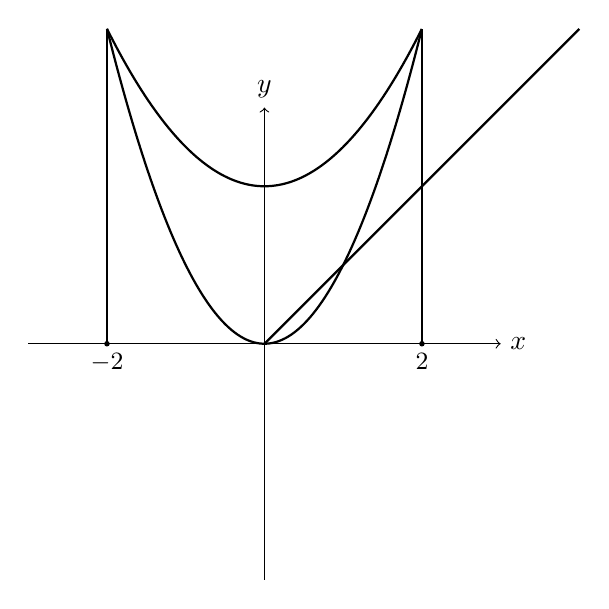
\begin{tikzpicture}
                \draw[black, thick, domain=-2:2, samples=100] 
                plot ({\x}, {((\x)^2}); 
                \draw[black, thick, domain=-2:2, samples=100] 
                plot ({\x}, {(0.5*(\x)^2 + 2});
                \draw[black, thick, domain=0:4, samples=100] 
                plot ({-2}, {((\x)});
                \draw[black, thick, domain=0:4, samples=100] 
                plot ({2}, {((\x)});
                \draw[black, thick, domain=0:4, samples=100] 
                plot ({\x}, {((\x)});
                \draw[->] (-3, 0) -- (3, 0) node[right] {$x$}; 
                \draw[->] (0, -3) -- (0, 3) node[above] {$y$};	
                \fill[black] (-2, 0) circle (1pt) node[below] {\small $-2$};
                \fill[black] (2, 0) circle (1pt) node[below] {\small $2$};
            \end{tikzpicture}
        }
        \end{center}
